\documentclass[aspectratio=169,10pt]{beamer}

\usetheme{Madrid}
\usecolortheme{default}
\setbeamertemplate{navigation symbols}{}
\setbeamertemplate{caption}[numbered]
\setbeamertemplate{footline}[frame number]

\usepackage{amsmath,amssymb}
\usepackage{booktabs}
\usepackage{graphicx}

\graphicspath{{./}}

\newcommand{\R}{\mathbb{R}}
\newcommand{\C}{\mathbb{C}}
\newcommand{\Koop}{\mathcal{K}}
\newcommand{\ii}{\mathrm{i}}

\title[Koopman Analysis of Chua's Circuit]{Koopman Analysis of Chua's Circuit with EDMD}
\subtitle{A data-driven spectral view of fixed points, periodic motion, period doubling, and chaos}
\author{Nonlinear Dynamics and Chaos Project}
\institute{}
\date{}

\begin{document}

\begin{frame}
    \titlepage
\end{frame}

\begin{frame}{Talk Roadmap}
    \begin{columns}[T,onlytextwidth]
        \begin{column}{0.52\textwidth}
            \begin{enumerate}
                \item Why Koopman operators are useful for nonlinear dynamics
                \item How EDMD approximates the Koopman operator from data
                \item Chua's circuit as an experimental route to chaos
                \item What the Koopman spectrum and eigenfunctions reveal
            \end{enumerate}
        \end{column}
        \begin{column}{0.43\textwidth}
            \begin{block}{Main takeaway}
                Koopman analysis does not make the circuit linear in state space.
                It finds nonlinear observables whose evolution is approximately linear,
                giving interpretable spectral structure across regimes.
            \end{block}
        \end{column}
    \end{columns}
\end{frame}

\begin{frame}{Motivation: Linear Tools for Nonlinear Motion}
    \begin{columns}[T,onlytextwidth]
        \begin{column}{0.48\textwidth}
            \textbf{Linear systems}
            \begin{itemize}
                \item Eigenvalues describe growth, decay, and oscillation
                \item Modes decompose the observed motion
                \item Spectra are compact summaries of dynamics
            \end{itemize}
        \end{column}
        \begin{column}{0.48\textwidth}
            \textbf{Nonlinear systems}
            \begin{itemize}
                \item Fixed points, cycles, bifurcations, and chaos
                \item No global linear modal decomposition in state coordinates
                \item Geometry may be hidden in nonlinear combinations of states
            \end{itemize}
        \end{column}
    \end{columns}

    \vspace{0.45cm}
    \begin{block}{Koopman idea}
        Instead of evolving the state directly, evolve observables of the state.
    \end{block}
\end{frame}

\begin{frame}{The Koopman Operator}
    For a discrete-time system
    \[
        x_{n+1} = F(x_n), \qquad x_n \in \R^d,
    \]
    an observable is a function \(g:\R^d \to \C\). The Koopman operator acts by composition:
    \[
        (\Koop g)(x) = g(F(x)).
    \]

    \vspace{0.25cm}
    \begin{columns}[T,onlytextwidth]
        \begin{column}{0.48\textwidth}
            \begin{block}{Key property}
                \[
                    \Koop(a g_1 + b g_2)
                    = a\Koop g_1 + b\Koop g_2.
                \]
                The operator is linear even when \(F\) is nonlinear.
            \end{block}
        \end{column}
        \begin{column}{0.48\textwidth}
            \begin{block}{Price paid}
                \(\Koop\) acts on a function space, which is generally infinite-dimensional.
            \end{block}
        \end{column}
    \end{columns}
\end{frame}

\begin{frame}{What Koopman Eigenfunctions Mean}
    A Koopman eigenfunction satisfies
    \[
        \Koop \xi_k = \lambda_k \xi_k,
        \qquad
        \xi_k(x_{n+1}) = \lambda_k \xi_k(x_n).
    \]

    \vspace{0.15cm}
    Therefore,
    \[
        \xi_k(x_n) = \lambda_k^n \xi_k(x_0).
    \]

    \vspace{0.2cm}
    \begin{columns}[T,onlytextwidth]
        \begin{column}{0.32\textwidth}
            \begin{block}{\(|\lambda| < 1\)}
                decay toward an attracting set
            \end{block}
        \end{column}
        \begin{column}{0.32\textwidth}
            \begin{block}{\(|\lambda| \approx 1\)}
                sustained oscillation or phase-like behavior
            \end{block}
        \end{column}
        \begin{column}{0.32\textwidth}
            \begin{block}{\(\arg(\lambda)\)}
                angular frequency per sample
            \end{block}
        \end{column}
    \end{columns}

    \vspace{0.25cm}
    \begin{alertblock}{Interpretation}
        The state can behave nonlinearly while an eigenfunction coordinate evolves by scalar multiplication.
    \end{alertblock}
\end{frame}

\begin{frame}{A Small Exact Example}
    Consider
    \[
        \dot{x}_1 = \mu x_1,
        \qquad
        \dot{x}_2 = \lambda(x_2 - x_1^2).
    \]
    In the original state variables the system is nonlinear, but the lifted observable vector
    \[
        \psi(x) =
        \begin{bmatrix}
            x_1 & x_2 & x_1^2
        \end{bmatrix}^{\top}
    \]
    evolves linearly:
    \[
        \frac{d}{dt}
        \begin{bmatrix}
            x_1 \\ x_2 \\ x_1^2
        \end{bmatrix}
        =
        \begin{bmatrix}
            \mu & 0 & 0 \\
            0 & \lambda & -\lambda \\
            0 & 0 & 2\mu
        \end{bmatrix}
        \begin{bmatrix}
            x_1 \\ x_2 \\ x_1^2
        \end{bmatrix}.
    \]

    \vspace{0.1cm}
    This is the ideal case EDMD tries to approximate from data.
\end{frame}

\begin{frame}{EDMD: Koopman from Snapshot Data}
    Choose a finite dictionary of observables
    \[
        \psi(x) =
        \begin{bmatrix}
            \psi_1(x) & \psi_2(x) & \cdots & \psi_{N_\psi}(x)
        \end{bmatrix}^{\top}.
    \]

    Given consecutive snapshot pairs \((x_k,x_{k+1})\),
    \[
        \Psi_X =
        \begin{bmatrix}
            \psi(x_1) & \cdots & \psi(x_M)
        \end{bmatrix},
        \qquad
        \Psi_Y =
        \begin{bmatrix}
            \psi(x_2) & \cdots & \psi(x_{M+1})
        \end{bmatrix}.
    \]

    EDMD solves
    \[
        \Psi_Y \approx K \Psi_X.
    \]

    \vspace{0.15cm}
    \begin{block}{In this project}
        \(K\) was computed by least squares with truncated SVD regularization; its eigenvalues, modes, and left eigenvectors approximate Koopman spectral data.
    \end{block}
\end{frame}

\begin{frame}{Experimental System: Chua's Circuit}
    \begin{columns}[T,onlytextwidth]
        \begin{column}{0.44\textwidth}
            \begin{itemize}
                \item Canonical nonlinear circuit with a piecewise-linear Chua diode
                \item Potentiometers used as bifurcation parameters
                \item Arduino R4 Minima sampled three conditioned voltages \(x,y,z\)
                \item Four regimes, \(5000\) samples each, roughly \(30\) kHz
            \end{itemize}
        \end{column}
        \begin{column}{0.52\textwidth}
            \centering
            \includegraphics[height=0.67\textheight]{ChuaCircuit.png}
        \end{column}
    \end{columns}
\end{frame}

\begin{frame}{Chua's Circuit: Governing Equations}
    \begin{columns}[T,onlytextwidth]
        \begin{column}{0.50\textwidth}
            Three coupled ODEs in \(x=V_{C_1},\,y=V_{C_2},\,z=I_L\):
            \[
                \dot x=\alpha[y-x-f(x)]
            \]
            \[
                RC_2\dot y=x-y+R_z
            \]
            \[
               \dot z =-\beta y
            \]

            \vspace{0.2cm}
            Piecewise-linear Chua diode characteristic:
            \[
                f(x) = G_b x
                  + \frac{G_a-G_b}{2}
                    \bigl(|x+E|-|x-E|\bigr)
            \]

            \vspace{0.15cm}
        \end{column}
        \begin{column}{0.46\textwidth}
            \centering
            
\includegraphics[height=0.5\textheight]{writeup/KppmanChuaCircuitDiagram.png}

            \vspace{0.05cm}
            {\footnotesize Phase portraits \(x\)--\(y\) across four regimes.}
        \end{column}
    \end{columns}
    \begin{block}{Our implementation}
        Inductor realized as a \textbf{gyrator} (two op-amps); Chua diode also op-amp based. Summing amplifiers shift bipolar voltages into the Arduino ADC window \([0,5]\,\mathrm{V}\).
    \end{block}
\end{frame}

\begin{frame}{Chua's Circuit: Dynamical Characteristics}
    \begin{columns}[T,onlytextwidth]
        \begin{column}{0.50\textwidth}
            \textbf{Bifurcation route} (resistance \(R\) via potentiometer):
            \[
                \text{fixed pt}
                \;\xrightarrow{\;R\downarrow\;}\;
                \text{limit cycle}
                \;\to\;
                \text{period-}\!2
                \;\to\;
                \text{chaos}
            \]
            \textbf{Measured Lyapunov spectrum} (double scroll, per sample):
            \[
                [\lambda_1,\,\lambda_2,\,\lambda_3]
                = [+0.084,\; -0.008,\; -1.223]
            \]
            \[
                \lambda_1^{\mathrm{ODE}} = +0.280
                \quad(\text{theory: }0.23)
            \]
            \textbf{Measured fractal dimensions} (double scroll):
            \begin{center}
                \small
                \begin{tabular}{lcc}
                    \toprule
                    & \(D_{\mathrm{box}}\) & \(D_{\mathrm{corr}}\) \\
                    Fixed point     & 0.161 & 0.696 \\
                    Limit cycle     & 1.101 & 1.067 \\
                    Period-doubled  & 1.052 & 1.214 \\
                    \textbf{Double scroll}  & \textbf{1.519} & \textbf{1.302} \\
                    \bottomrule
                \end{tabular}
            \end{center}
            {\footnotesize Underestimates of \(\approx 2.07\) expected at \(N=5000\) pts.}
        \end{column}
        \begin{column}{0.46\textwidth}
            \begin{block}{Data collection}
                \begin{itemize}
                    \item Four regimes, \(5000\) samples each
                    \item \(\approx 30\,\mathrm{kHz}\) via direct ADC
                          register reads on the R4 Minima
                          (bypasses \texttt{analogRead()} overhead)
                    \item Signals: \(x = V_{C_1},\;
                                    y = V_{C_2},\;
                                    z = I_L\)
                    \item Consecutive snapshot pairs
                          \((x_k, x_{k+1})\) passed directly to EDMD
                \end{itemize}
            \end{block}
           
            \vspace{0.2cm}
            \begin{block}{\(D_{\mathrm{box}} > 1\) confirms strange attractor}
                Non-integer dimension between 1 and 2 signals a fractal
                geometric structure; underestimate of \(\approx 2.07\)
                expected at \(N=5000\) pts (reliable scaling requires
                \(\sim 10^{D}\) points).
            \end{block}
        \end{column}
    \end{columns}
\end{frame}

\begin{frame}{Lyapunov Spectrum Across All Regimes}
    \begin{columns}[T,onlytextwidth]
        \begin{column}{0.54\textwidth}
            \centering
            \includegraphics[width=\textwidth,height=0.72\textheight,keepaspectratio]%
                {/chua_analysis/chua_lyapunov_bar.png}
        \end{column}
        \begin{column}{0.42\textwidth}
            \textbf{Reading the spectrum:}
            \begin{itemize}
                \item \(\lambda_1 < 0\): all directions contract
                      \(\Rightarrow\) \textbf{fixed point} (globally stable)
                \item \(\lambda_1 \approx 0,\;\lambda_2,\lambda_3 < 0\):
                      one neutral direction along the orbit
                      \(\Rightarrow\) \textbf{limit cycle}
                \item Same pattern, slightly less negative \(\lambda_1\):
                      \textbf{period-doubled} orbit (still periodic)
                \item \(\lambda_1 > 0\): exponential divergence
                      \(\Rightarrow\) \textbf{chaos}
            \end{itemize}

            \vspace{0.2cm}
           
        \end{column}
    \end{columns}
    \vspace{0.1cm}
        \begin{alertblock}{Double scroll}
            \([\lambda_1,\lambda_2,\lambda_3]
              = [+0.084,\;-0.008,\;-1.223]\)/sample, \(\lambda_1^{\mathrm{ODE}} = +0.280\)
            \;(theory: \(0.23\),\;\(\tau = R_{\mathrm{eff}}C_2 = 0.1\,\mathrm{ms}\))\\[3pt]
            Divergence time:\;
            \(T_{\mathrm{div}} = 1/\lambda_1 \approx 12\) samples
            \(\approx 0.40\,\mathrm{ms}\) \(\sim\tfrac{1}{4}\) of one oscillation period
            \(\Rightarrow\) strongly chaotic\\[3pt]
            \(\Rightarrow D_{\mathrm{box}} = 1.519\)
            \;(fractal; limited by \(N=5000\) pts)
        \end{alertblock}
\end{frame}

\begin{frame}{Measured Route to Chaos}
    \begin{columns}[T,onlytextwidth]
        \begin{column}{0.49\textwidth}
            \centering
            \textbf{Oscilloscope (raw experimental)}\\[0.2em]
            \begin{tabular}{@{}cc@{}}
                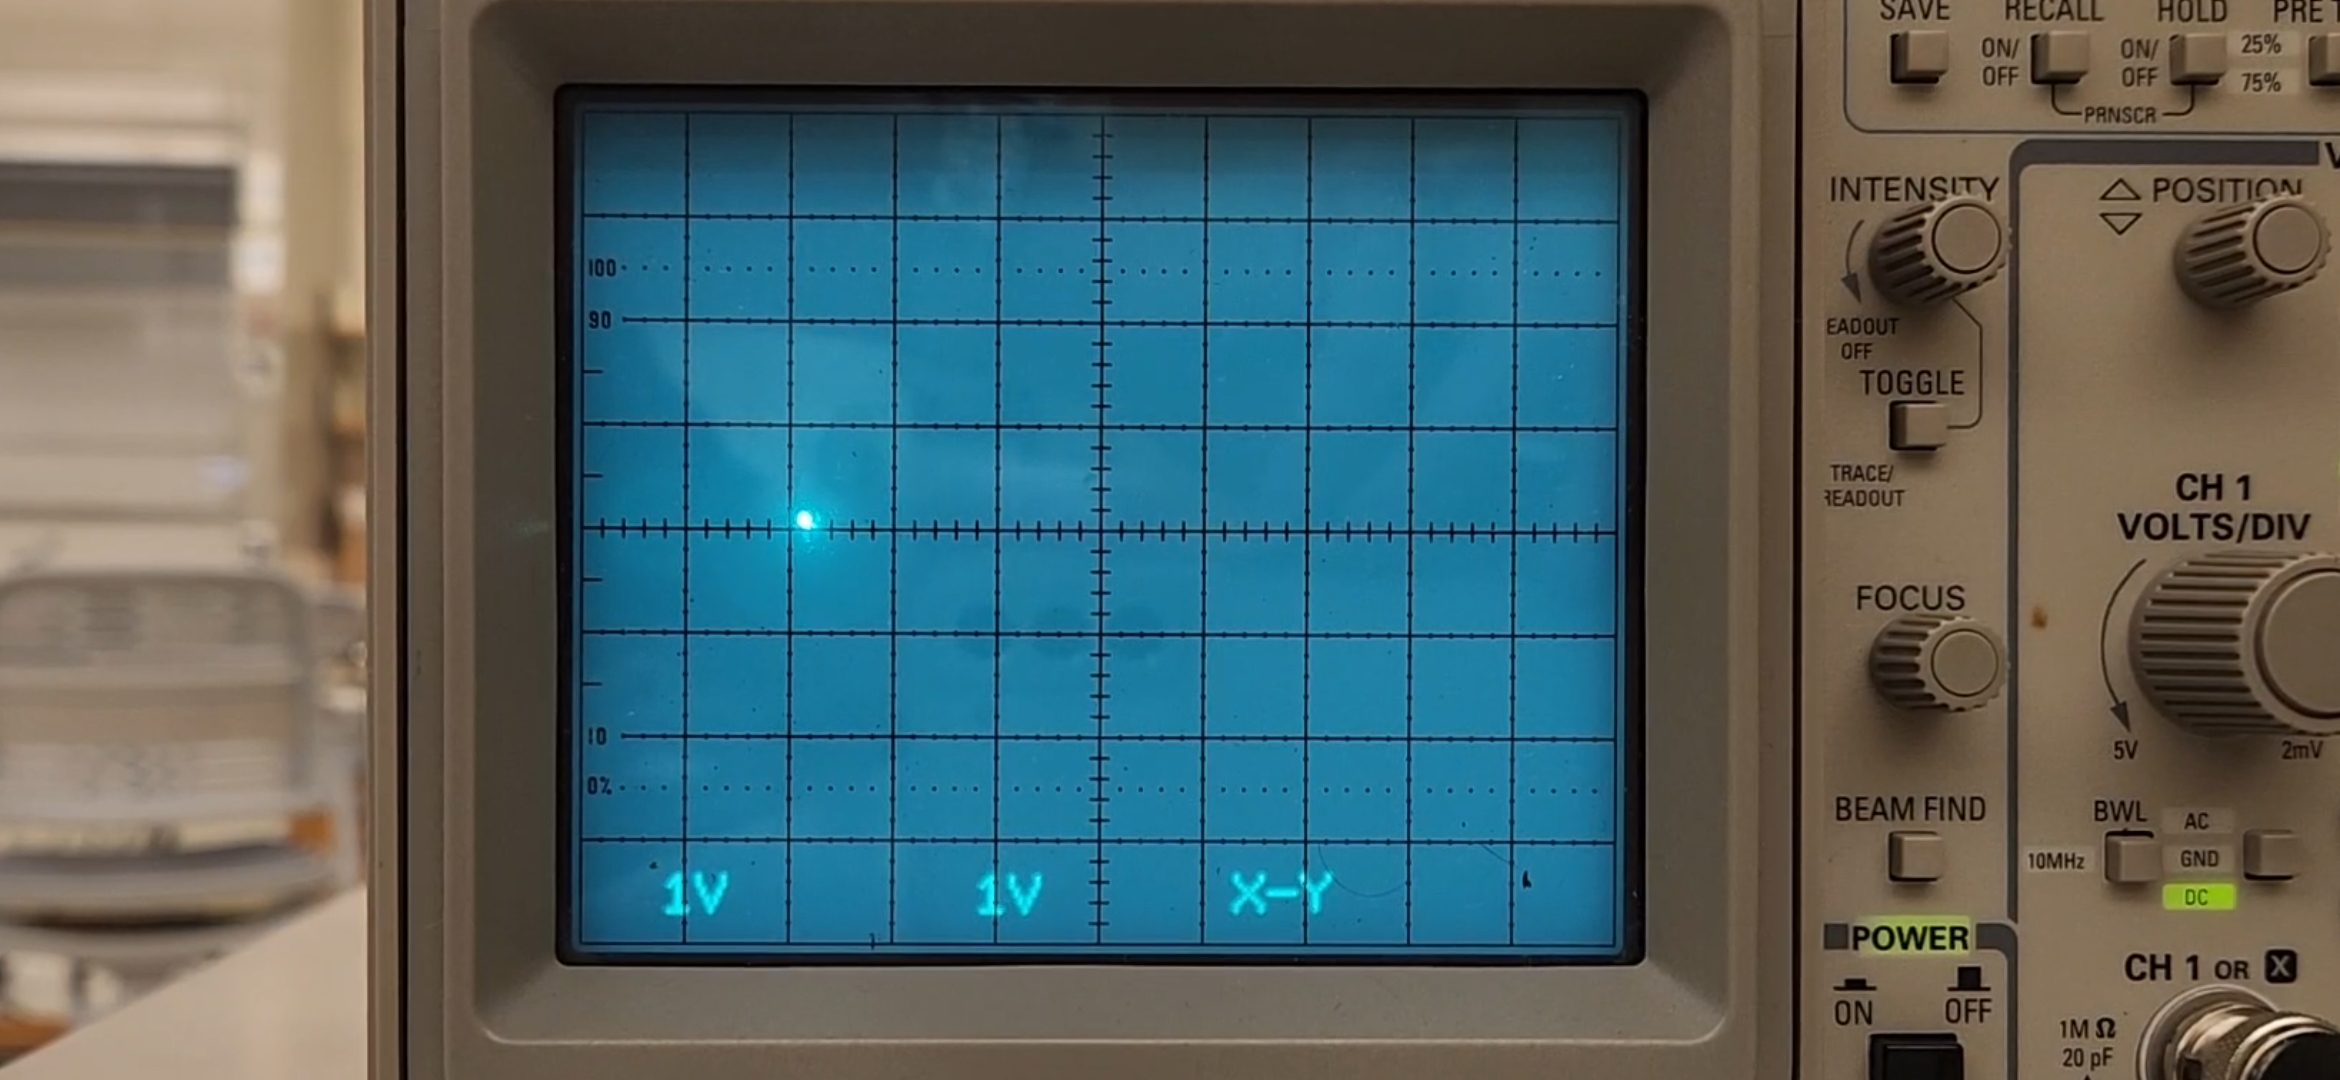
\includegraphics[width=0.46\linewidth]{oscilloscopePics/stableNode.jpg} &
                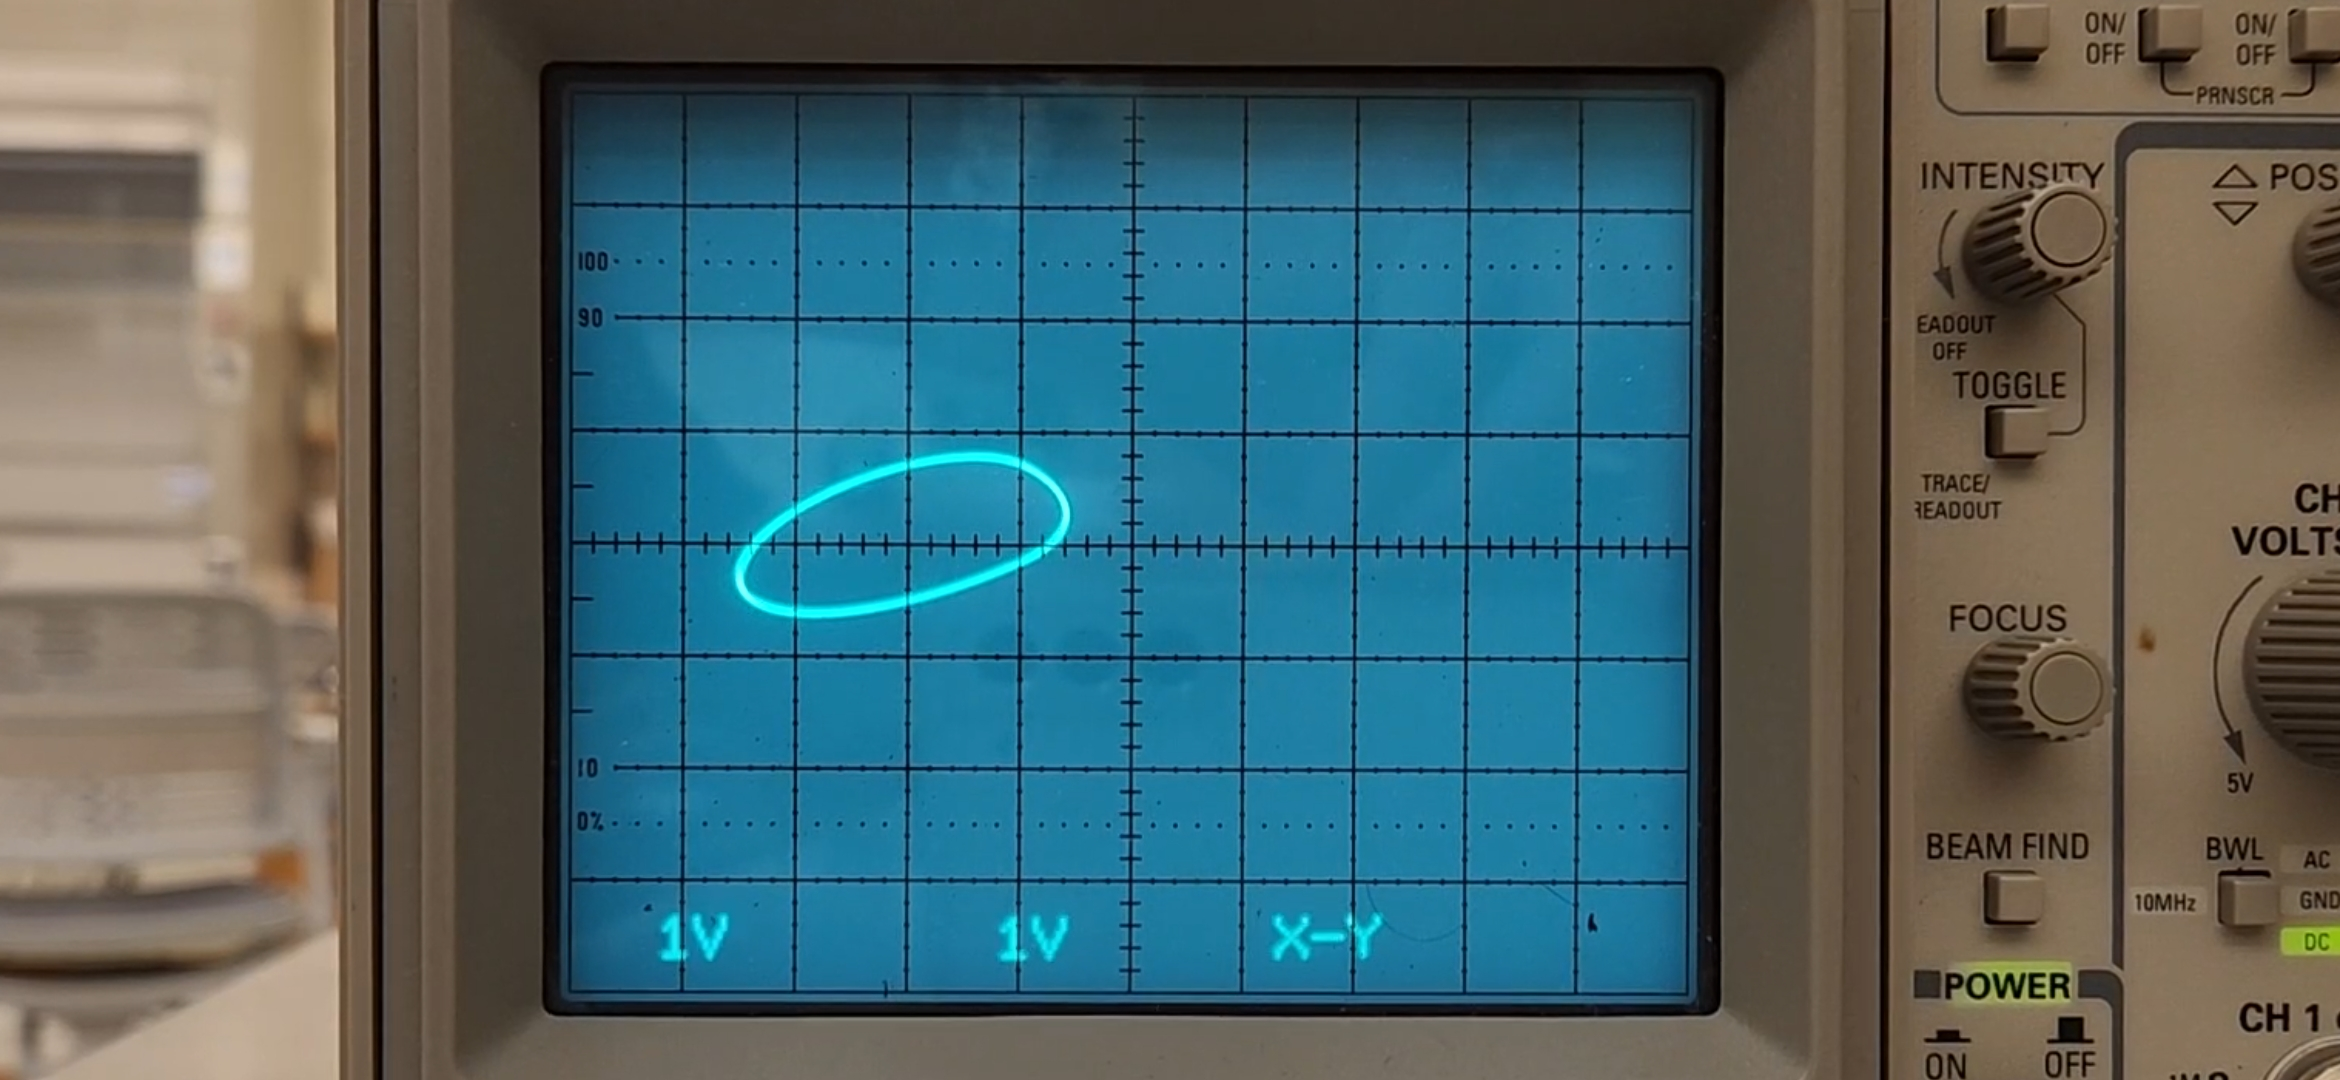
\includegraphics[width=0.46\linewidth]{oscilloscopePics/limitCycle.jpg} \\[-0.1em]
                {\scriptsize fixed point} & {\scriptsize limit cycle} \\
                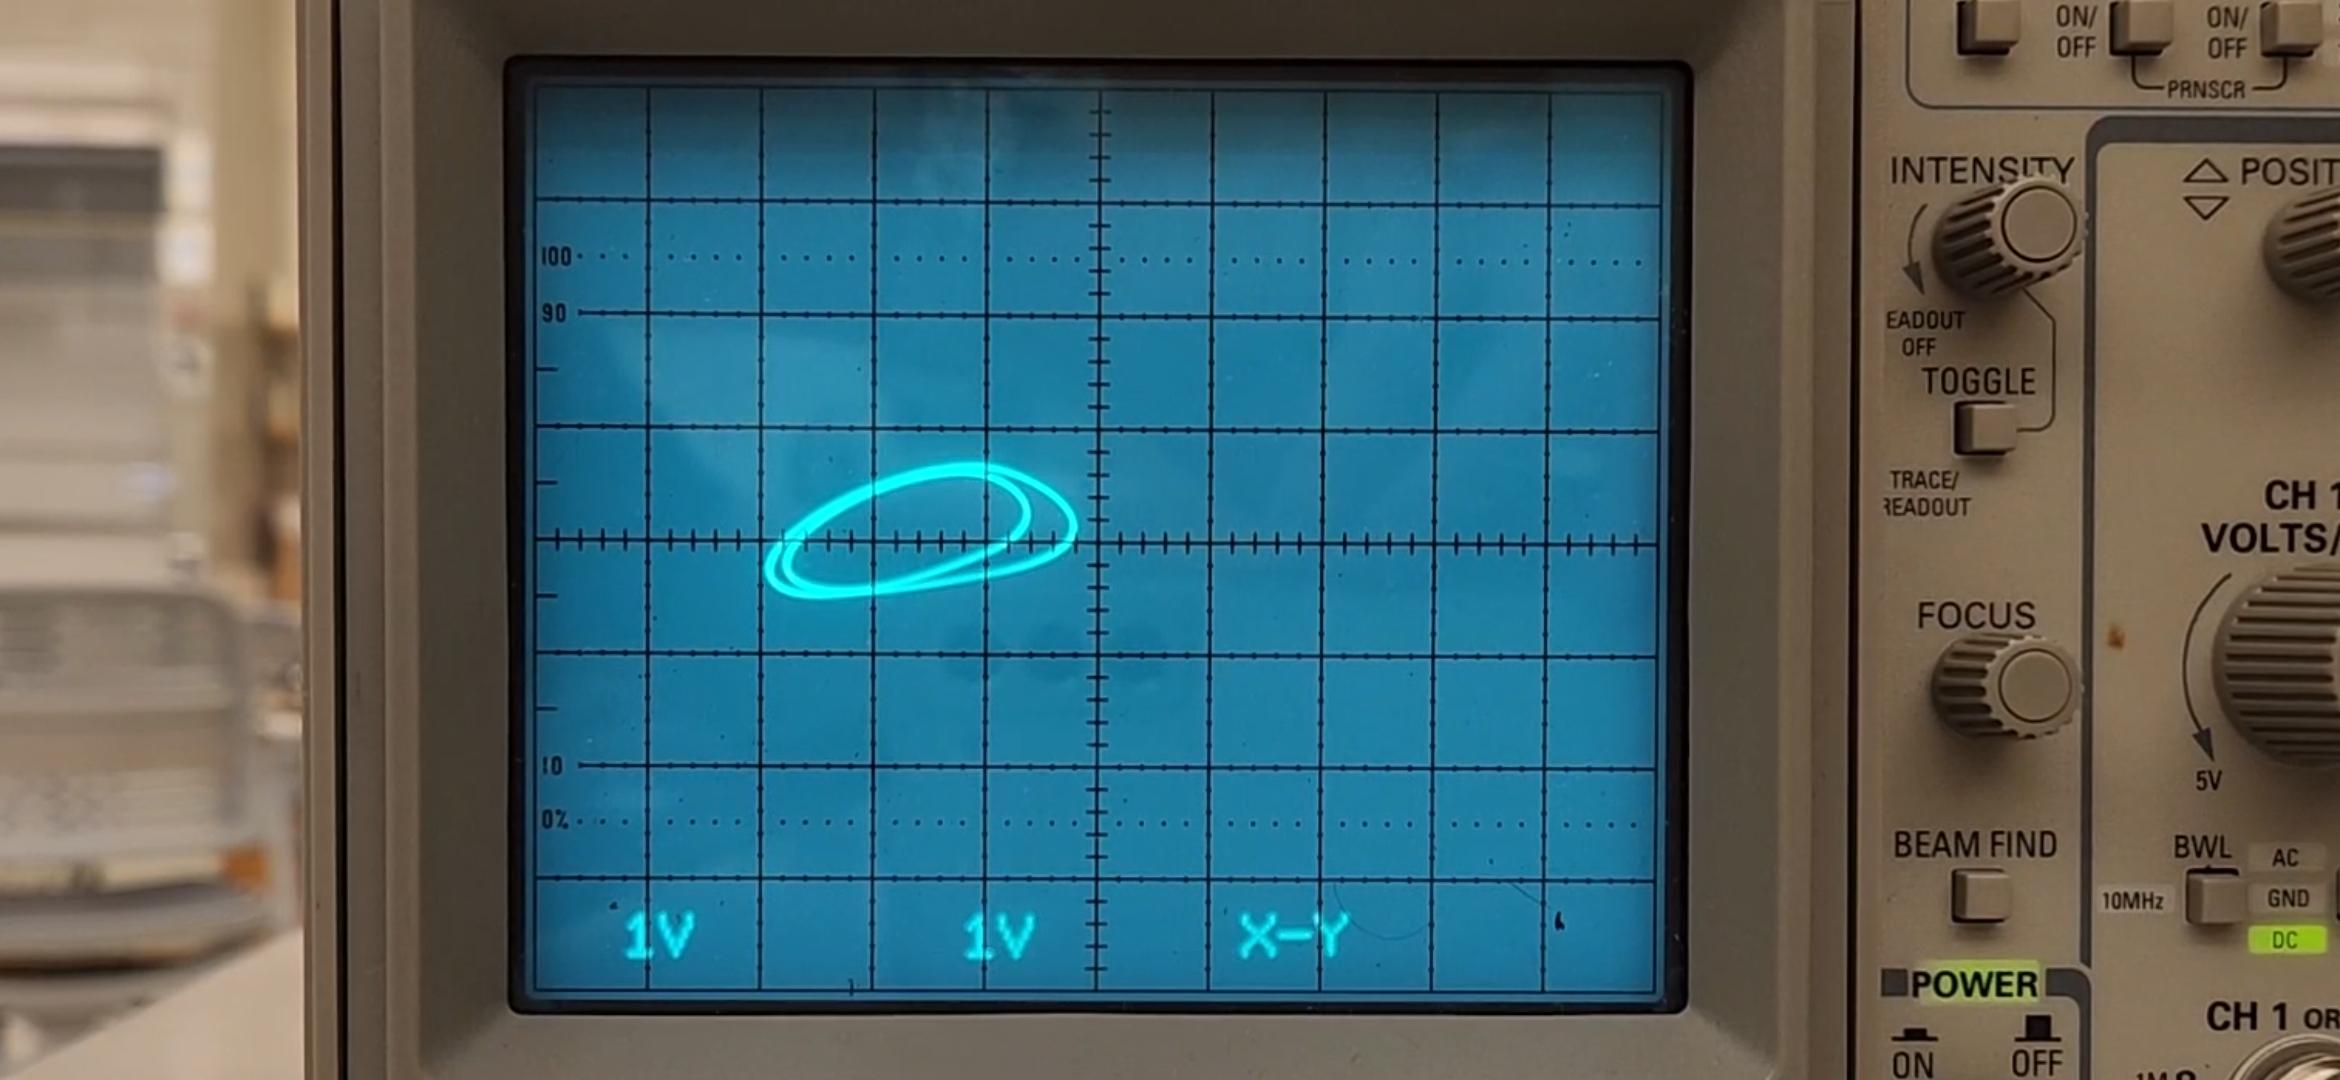
\includegraphics[width=0.46\linewidth]{oscilloscopePics/periodDoubled.jpg} &
                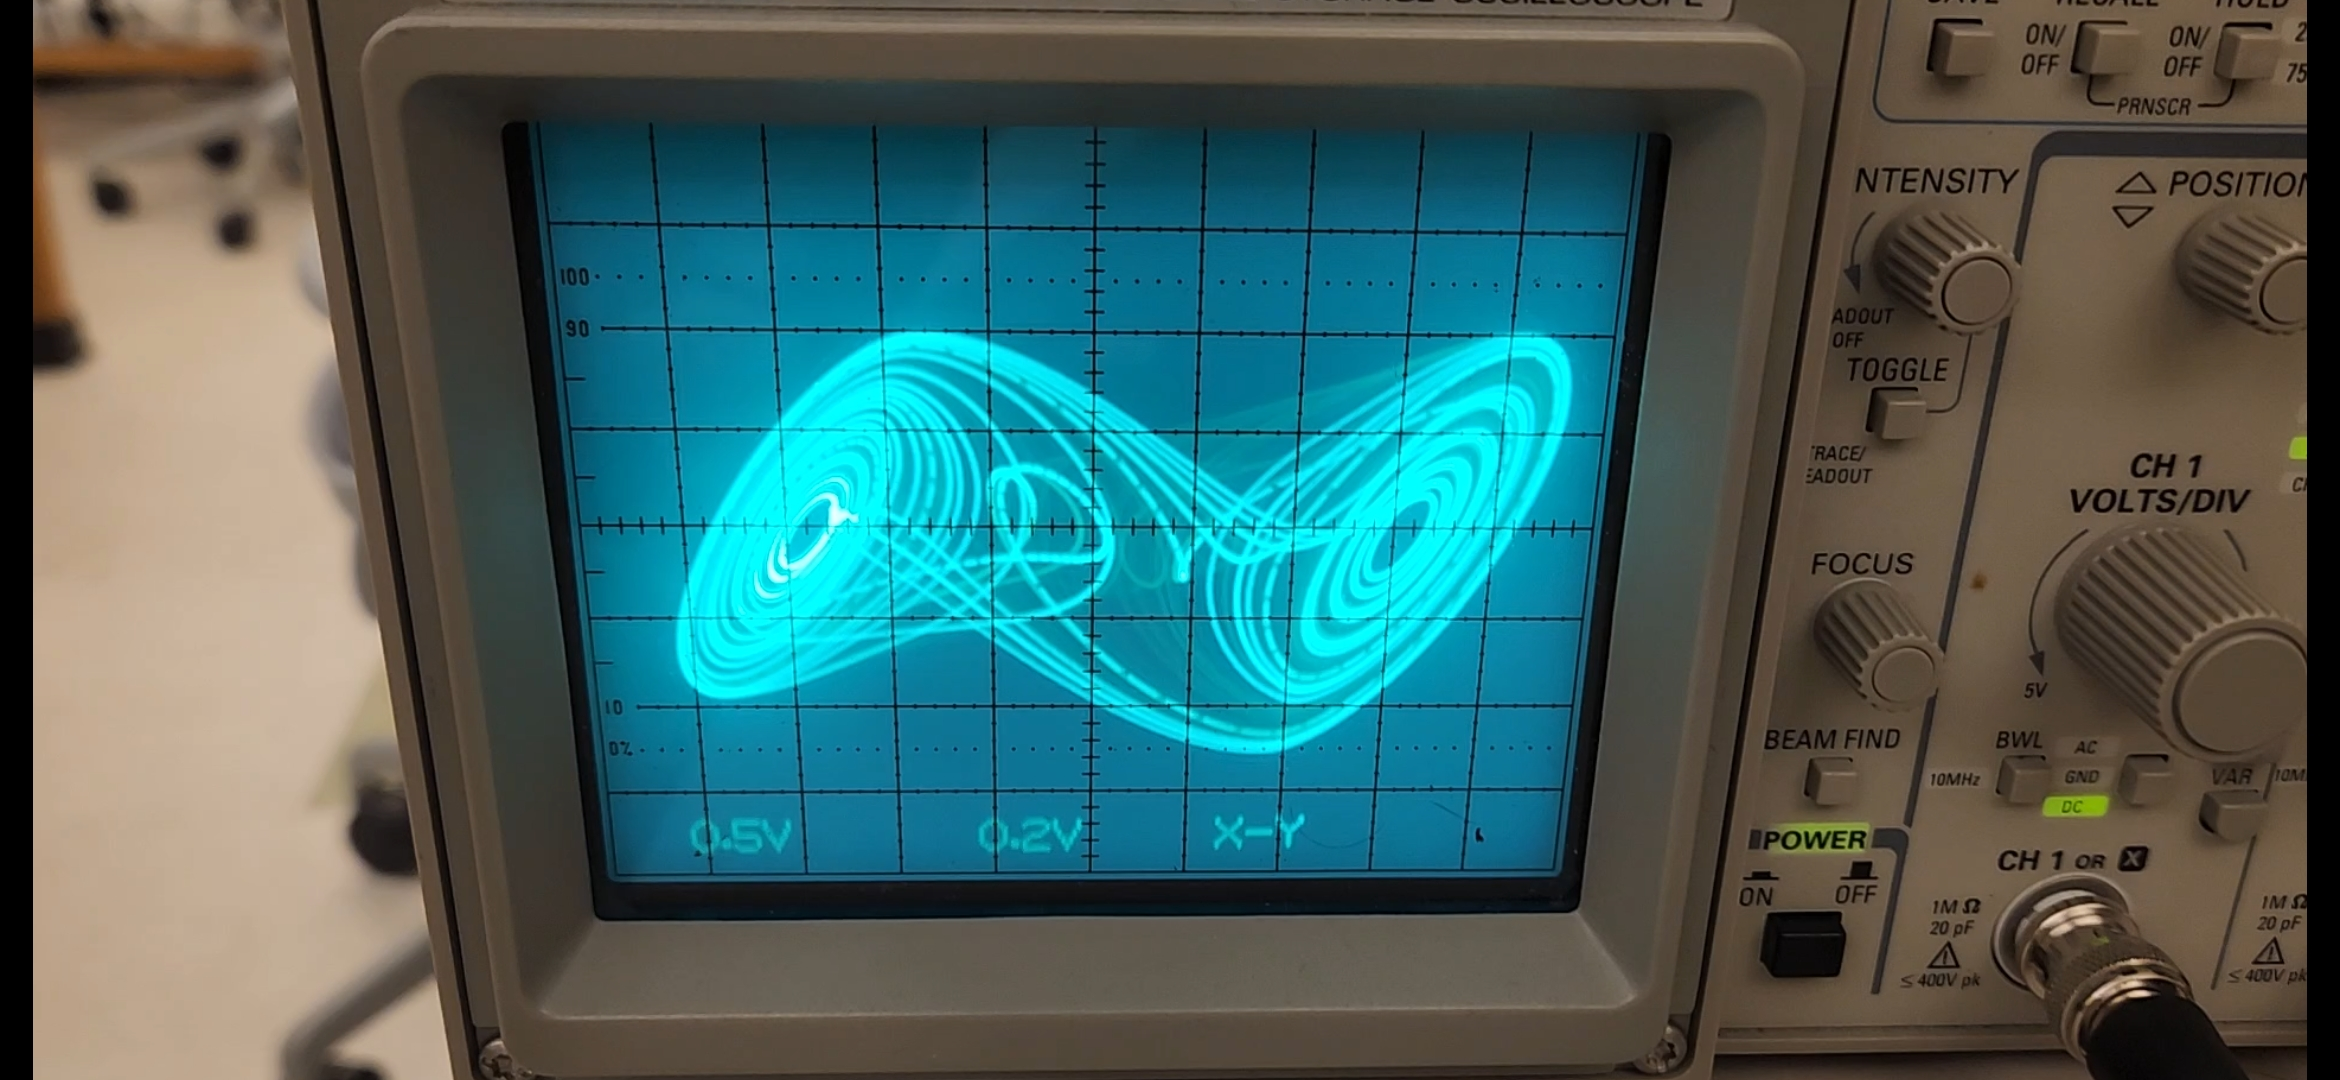
\includegraphics[width=0.46\linewidth]{oscilloscopePics/doubleScroll.jpg} \\[-0.1em]
                {\scriptsize period doubled} & {\scriptsize double scroll}
            \end{tabular}
        \end{column}
        \begin{column}{0.49\textwidth}
            \centering
            \textbf{Sampled phase portraits}\\[0.2em]
            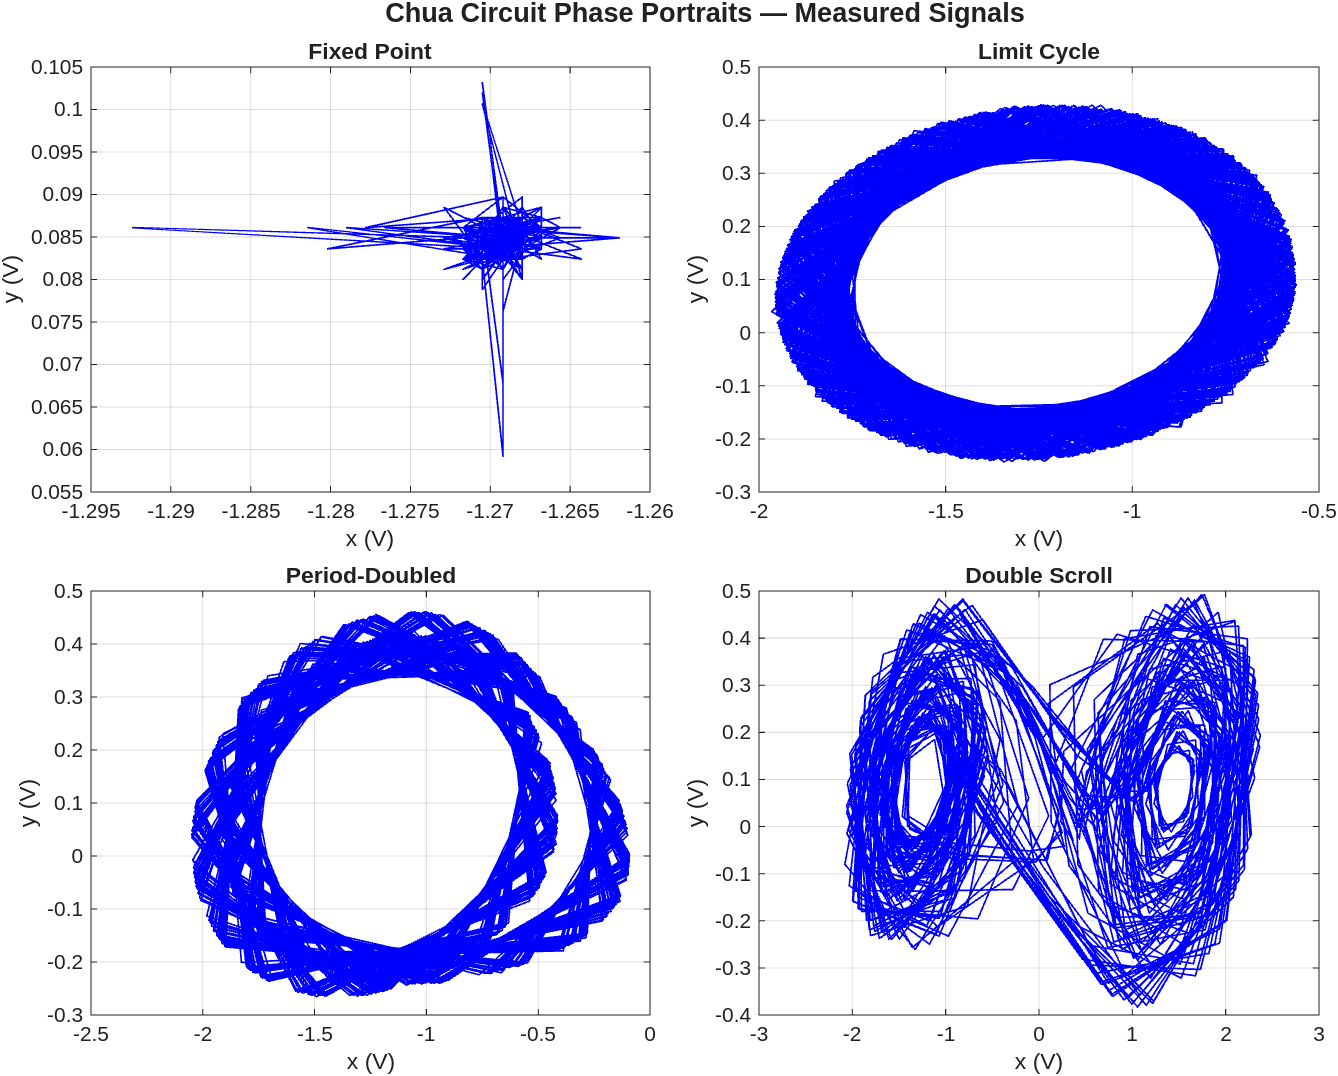
\includegraphics[width=\linewidth,height=0.72\textheight,keepaspectratio]{MeasuredChua.png}
        \end{column}
    \end{columns}

    \vspace{0.1cm}
    \centering
    {\small Fixed point \(\rightarrow\) limit cycle \(\rightarrow\) period-doubled orbit \(\rightarrow\) double-scroll chaos.}
\end{frame}

\begin{frame}{Dictionary Choice Matters}
    \begin{columns}[T,onlytextwidth]
        \begin{column}{0.42\textwidth}
            Dictionaries tested:
            \begin{itemize}
                \item Linear states
                \item Polynomial monomials
                \item Radial basis functions
                \item Chua-matched piecewise-linear kink terms
                \item Combined full dictionary
            \end{itemize}

            \vspace{0.15cm}
            Data were normalized to \([-1,1]\) before lifting.
        \end{column}
        \begin{column}{0.55\textwidth}
            \centering
            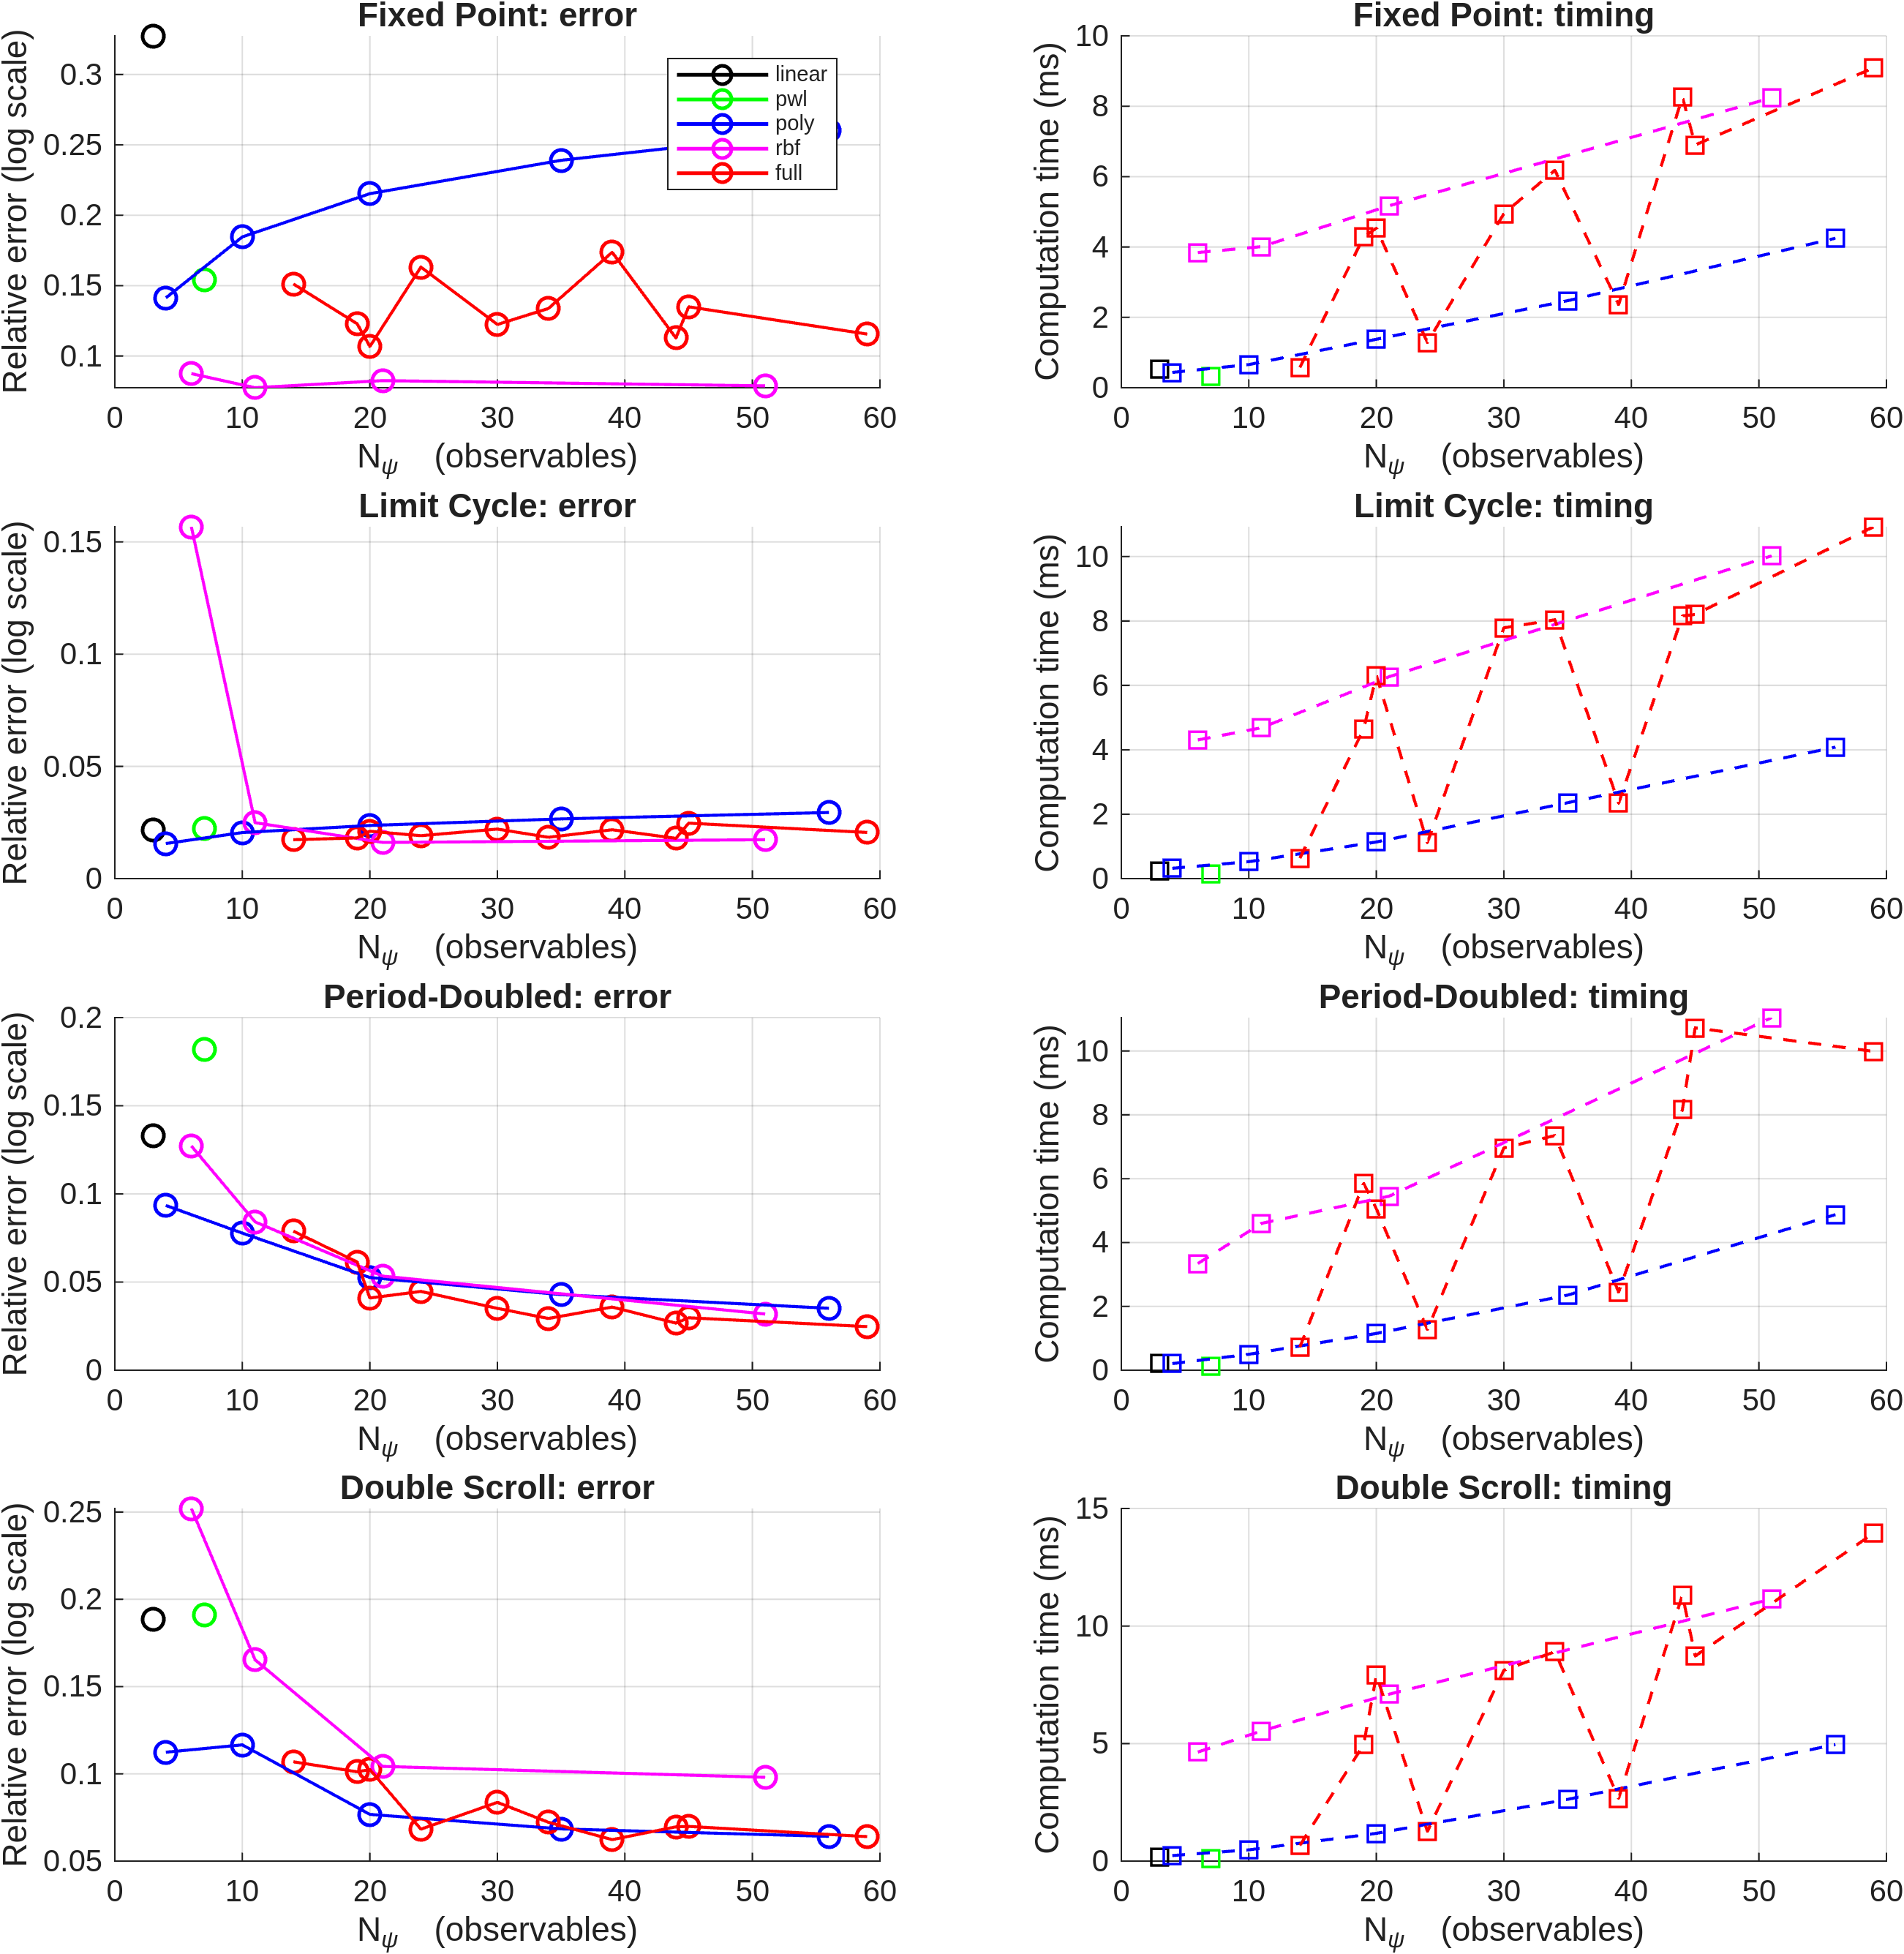
\includegraphics[width=\textwidth,height=0.75\textheight,keepaspectratio]{dictionarySweep.png}
        \end{column}
    \end{columns}
\end{frame}

\begin{frame}{Dictionary Sweep: Accuracy Versus Cost}
    \begin{columns}[T,onlytextwidth]
        \begin{column}{0.48\textwidth}
            \begin{block}{Accuracy}
                Richer dictionaries reduce lifted one-step error across regimes.
                The improvement is largest for the double-scroll data.
            \end{block}
        \end{column}
        \begin{column}{0.48\textwidth}
            \begin{block}{Cost}
                EDMD solve time increases with the number of observables \(N_\psi\);
                richer dictionaries are not free.
            \end{block}
        \end{column}
    \end{columns}

    \vspace{0.25cm}
    \begin{alertblock}{Practical conclusion}
        Koopman analysis is not automatic linearization. The observable dictionary has to match the dynamics.
    \end{alertblock}
\end{frame}

\begin{frame}{Koopman Eigenvalues Across Regimes}
    \centering
    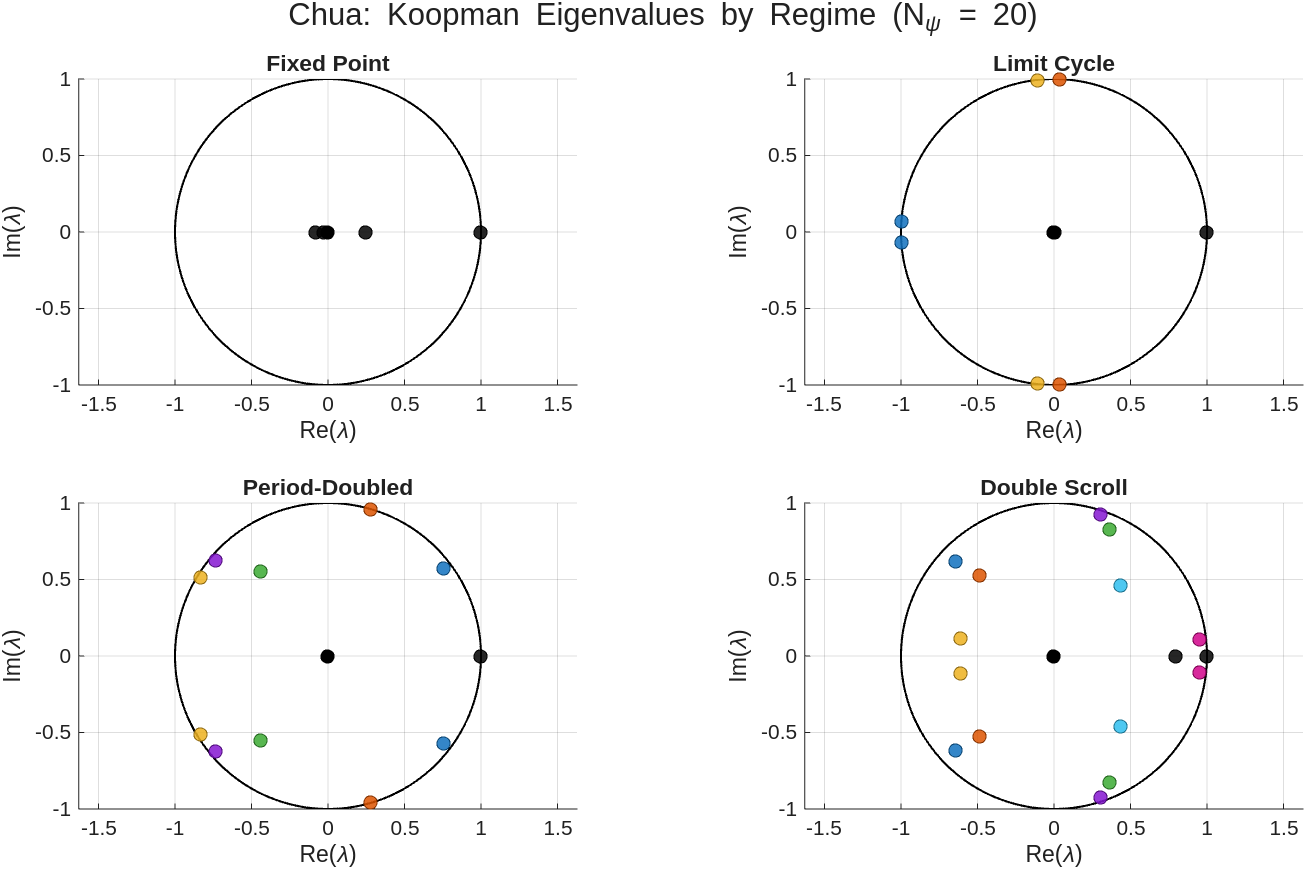
\includegraphics[width=0.82\textwidth,height=0.68\textheight,keepaspectratio]{eigenvalues.png}

    \vspace{0.05cm}
    Degree-3 polynomial dictionary, \(N_\psi=20\); unit circle shown for reference.
\end{frame}

\begin{frame}{Reading the Spectrum}
    \begin{columns}[T,onlytextwidth]
        \begin{column}{0.48\textwidth}
            \begin{block}{Fixed point}
                Real eigenvalues inside the unit circle: non-oscillatory decay.
            \end{block}
            \begin{block}{Limit cycle}
                Conjugate pairs near roots of unity: sustained periodic motion.
            \end{block}
        \end{column}
        \begin{column}{0.48\textwidth}
            \begin{block}{Period doubled}
                New intermediate-angle conjugate pairs: subharmonic content at half the original frequency.
            \end{block}
            \begin{block}{Double scroll}
                Broad spectrum on and inside the unit circle: no finite set of clean periodic frequencies captures the chaos.
            \end{block}
        \end{column}
    \end{columns}
\end{frame}

\begin{frame}{Period Doubling: Modes Reconstruct Geometry}
    \begin{columns}[T,onlytextwidth]
        \begin{column}{0.38\textwidth}
            \begin{itemize}
                \item Top Koopman modes ranked by contribution to \(x\)-state energy
                \item Oscillatory eigenvalues projected back to the unit circle to remove numerical decay
                \item Samples colored by the sign of the \(f_0/2\) eigenfunction
            \end{itemize}

            \vspace{0.15cm}
            \begin{block}{Result}
                Ten modes recover the two-loop topology of the period-doubled orbit.
            \end{block}
        \end{column}
        \begin{column}{0.58\textwidth}
            \centering
            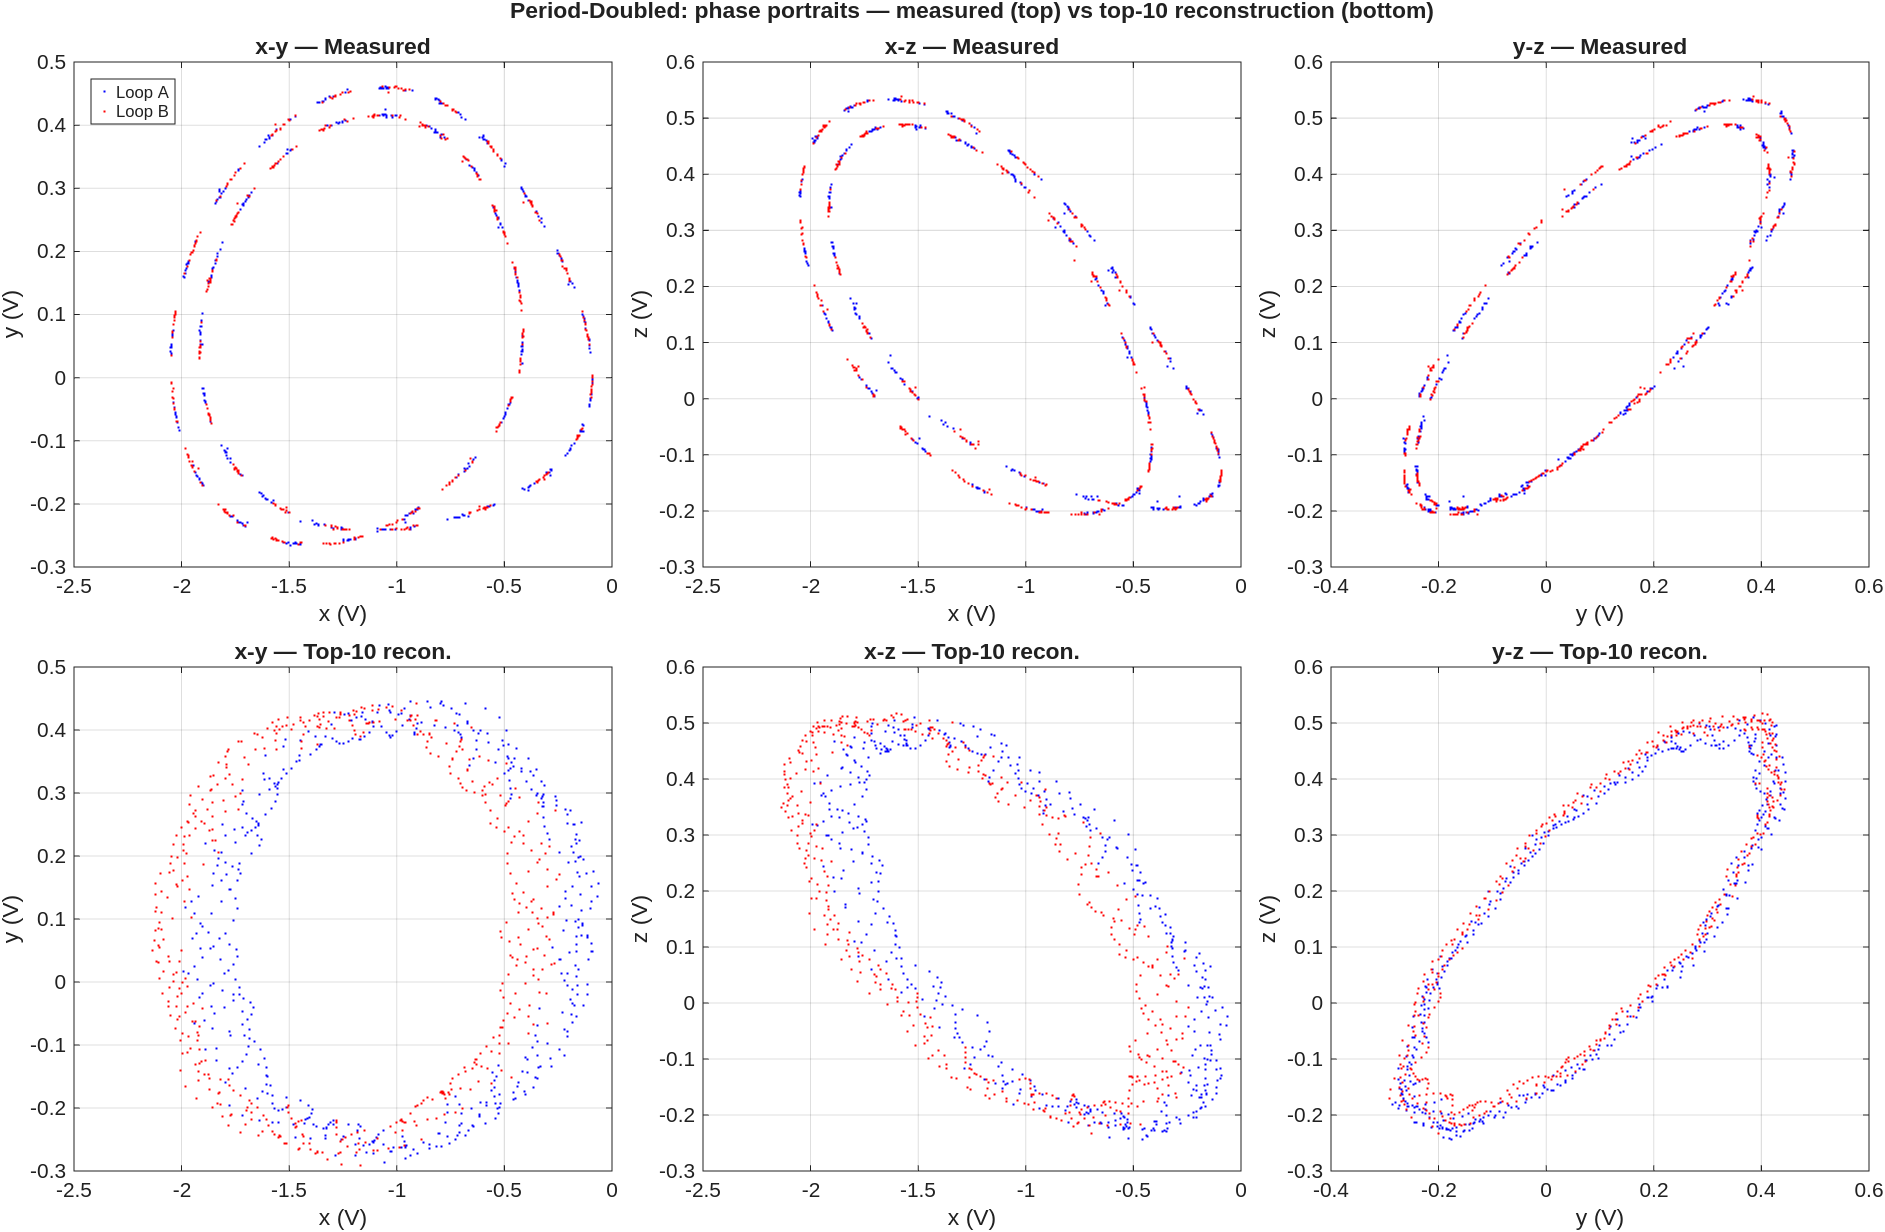
\includegraphics[width=\textwidth,height=0.72\textheight,keepaspectratio]{periodDoubledPP.png}
        \end{column}
    \end{columns}
\end{frame}

\begin{frame}{Double Scroll: Eigenfunctions as Hidden Coordinates}
    \begin{columns}[T,onlytextwidth]
        \begin{column}{0.38\textwidth}
            The selected eigenfunction had
            \[
                |\lambda_k| = 0.957,
                \qquad
                f_k \approx 605~\mathrm{Hz}.
            \]

            \begin{itemize}
                \item Phase of \(\xi_k\) gives smooth coloring around the lobes
                \item \(\operatorname{sign}(\operatorname{Re}\xi_k)\) separates the scrolls
                \item Real and imaginary parts show near-rotational evolution
            \end{itemize}
        \end{column}
        \begin{column}{0.58\textwidth}
            \centering
            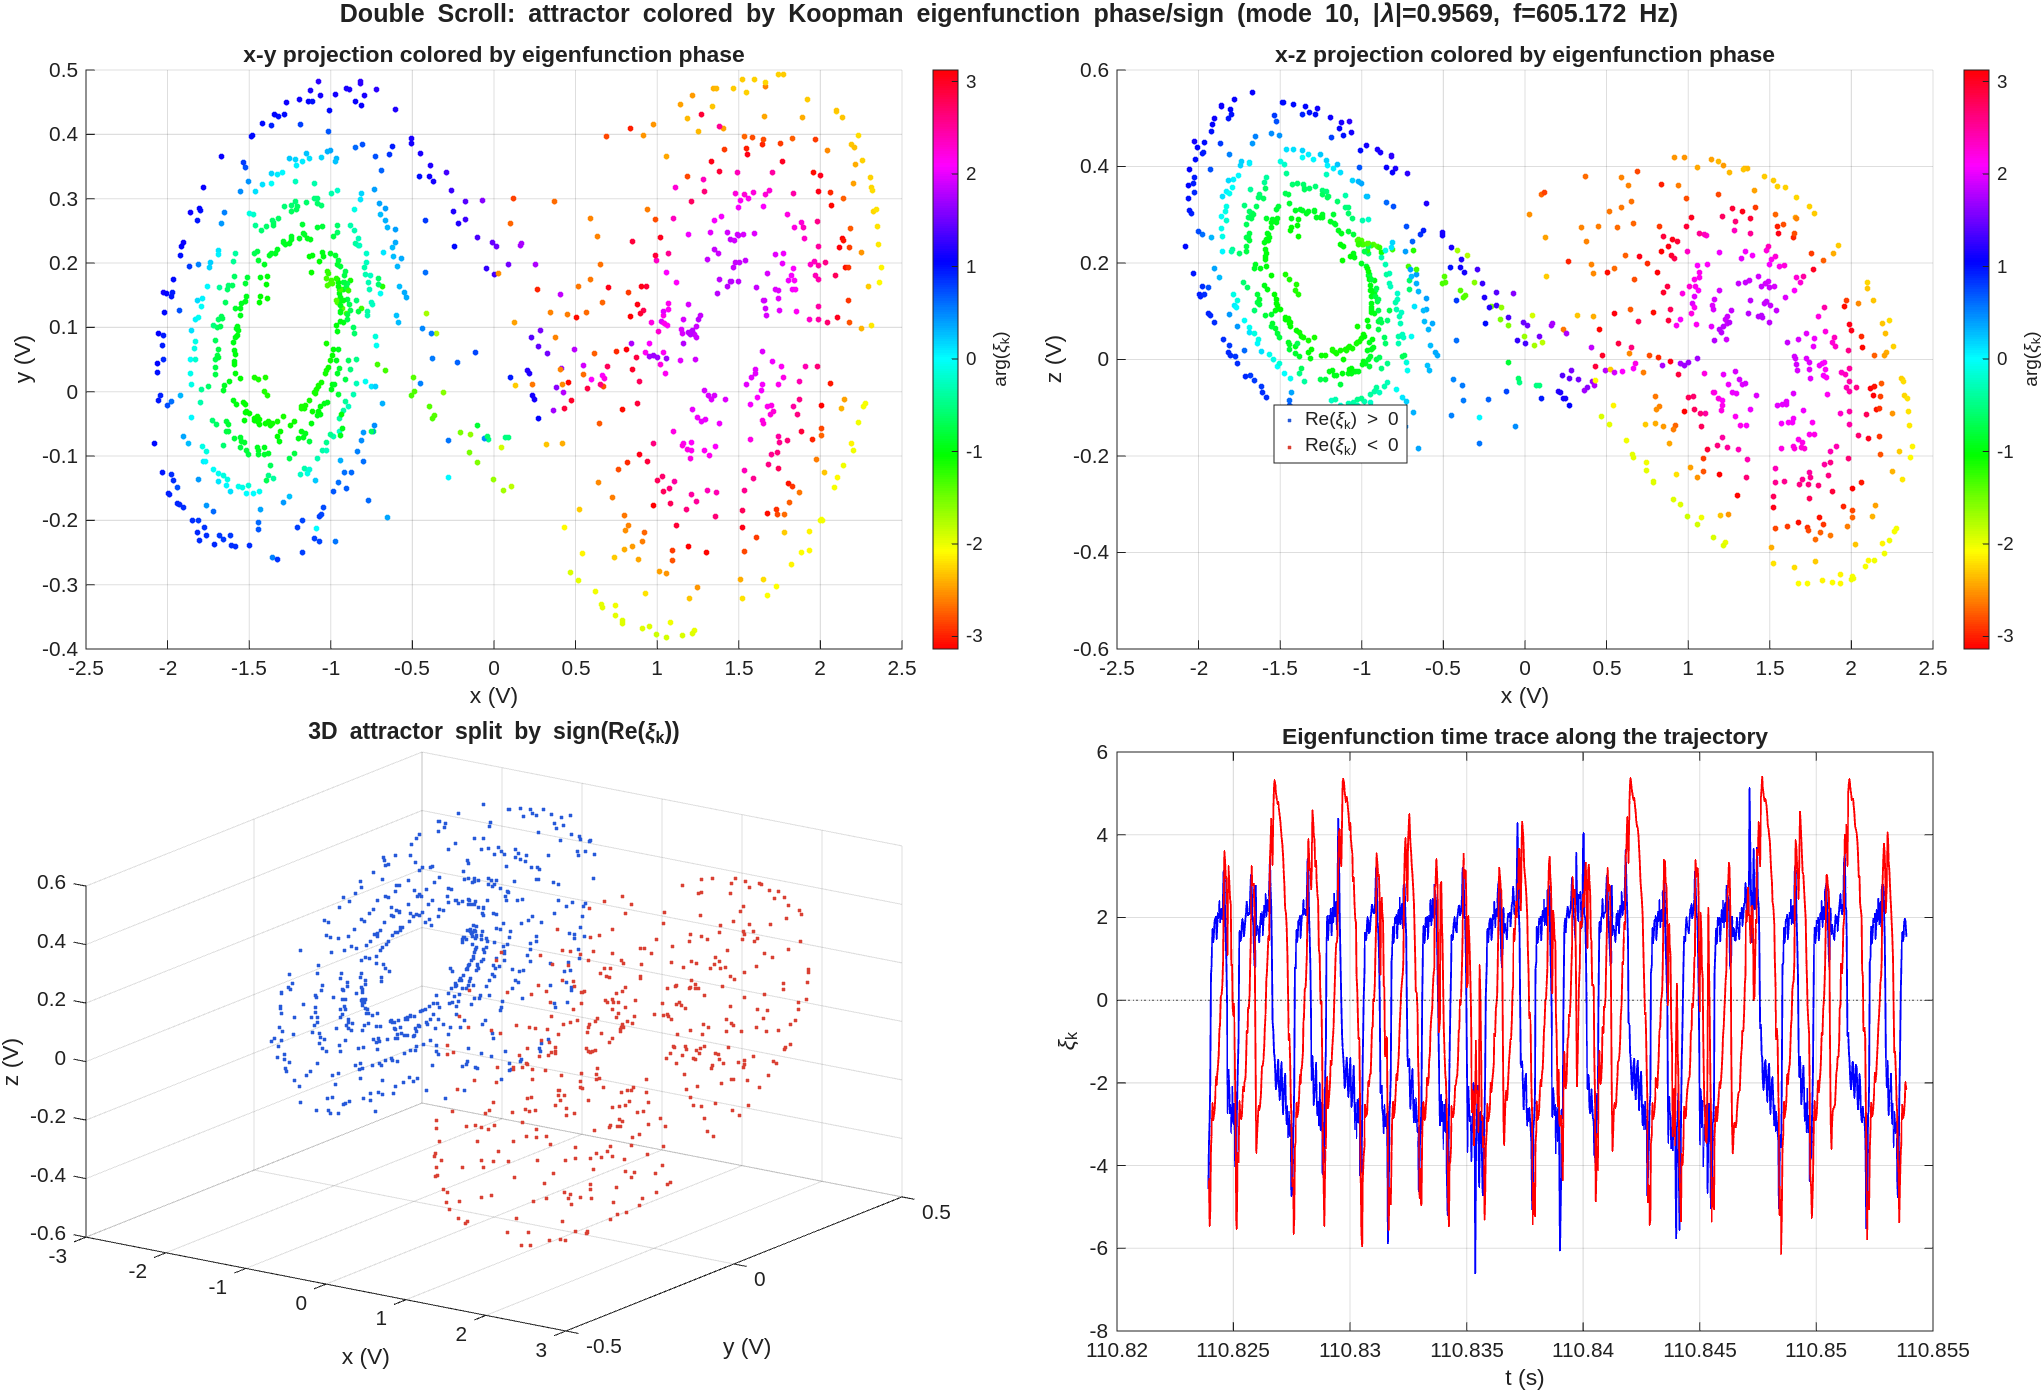
\includegraphics[width=\textwidth,height=0.73\textheight,keepaspectratio]{doubleScrollColoring.png}
        \end{column}
    \end{columns}
\end{frame}

\begin{frame}{Project Conclusions}
    \begin{enumerate}
        \item Koopman operators give a linear spectral language for nonlinear dynamics by lifting from states to observables.
        \item EDMD makes this practical from measured data, but the result depends strongly on dictionary choice.
        \item For Chua's circuit, Koopman spectra match the qualitative route to chaos:
        fixed point, limit cycle, period doubling, then double scroll.
        \item In the chaotic regime, eigenfunctions reveal coherent geometry that is not obvious in raw voltage coordinates.
    \end{enumerate}

    \vspace{0.25cm}
    \begin{alertblock}{Final takeaway}
        The Koopman viewpoint organizes the data: it identifies oscillatory content in periodic regimes and hidden coordinates on the chaotic attractor.
    \end{alertblock}
\end{frame}

\begin{frame}{References}
    \small
    \begin{thebibliography}{9}
        \bibitem{koopman1931}
        B. O. Koopman.
        \newblock Hamiltonian systems and transformation in Hilbert space.
        \newblock \emph{PNAS}, 1931.

        \bibitem{williams2015}
        M. O. Williams, I. G. Kevrekidis, and C. W. Rowley.
        \newblock A data-driven approximation of the Koopman operator: Extending dynamic mode decomposition.
        \newblock \emph{Journal of Nonlinear Science}, 2015.

        \bibitem{chua1986}
        L. O. Chua, M. Komuro, and T. Matsumoto.
        \newblock The double scroll family.
        \newblock \emph{IEEE Transactions on Circuits and Systems}, 1986.

        \bibitem{matsumoto1984}
        T. Matsumoto.
        \newblock A chaotic attractor from Chua's circuit.
        \newblock \emph{IEEE Transactions on Circuits and Systems}, 1984.
    \end{thebibliography}
\end{frame}

\begin{frame}{Largest Lyapunov Exponent --- Double Scroll}
    \centering
    \includegraphics[width=0.82\textwidth,height=0.78\textheight,keepaspectratio]%
        {/chua_analysis/chua_lyapunov_doublescroll.png}
\end{frame}

\end{document}
